\subsection{Hopfield Network}

% Wenting.
Hopfield's model is an associative(content-addressable) memory model using binary information and its network is featured with threshold and feedback. A binary input vector to a Hopfiled Network will be recursively processed(fed back) at the granularity level of bit, until a threshold criterium is met, the produced output vector possesses the feature that is with the shortest Hamming distance to its origin input vector (see figure \ref{fig:hopfield_network}). There properties give rise to associative memory recall, where an input pattern (i.e. memory cue) is presented to the Hopfield network, which produces an output vector that is closest in Hamming distance to a previously stored memory, thus filling in the gaps to recall a memory through association.

\begin{figure}[htbp]
	\begin{center}
		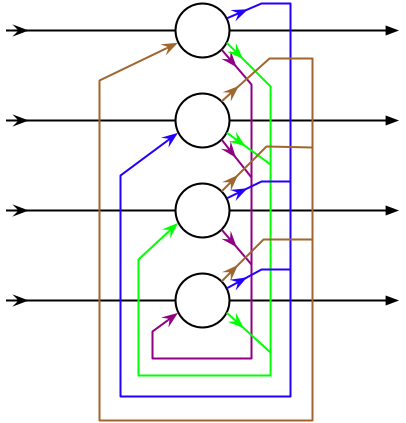
\includegraphics[width=0.5\textwidth]{inc/hopfield_network.png}
		\caption{A Hopfield network consisting of 4 nodes, with an input and output vector of length 4. Additionally, each node takes as input the state of each other node in the network.\protect\footnotemark}
		\label{fig:hopfield_network}
	\end{center}
\end{figure}
\footnotetext{Original image (CC BY-SA): \url{https://upload.wikimedia.org/wikipedia/commons/9/95/Hopfield-net.png}}

In paper from J.J.Hopfield(1982) \cite{computational_abilities}, the drawbacks of Perceptron were addressed through its intractable back-coupling, lack of abstraction properties and requirement of synchronism. Information storage was improved with help of Nonlinearity, and emergent computational properties were obtained from simple properties of many cells rather than complex circuitry(which is a result of linear associativity). The input-output relationship of nonlinear computation, binary threshold units and concept of the energy function were introduced.

Collective behaviors of the model was studied and resulted with the following findings: a few stable states was resulted from most of the initial state space, properties necessary for a physical content-addressable memory were not dependent on the symmetry of the connectivity matrix $T_{ij}$. Statement supported by findings from experiments is that ``about 0.15N(memory storage bits, number of neurons) states can be simultaneously remembered before error in recall is severe'', which refers to the memory capacity of the associative memory. Case with arbitrary starting state was studied and results of memories near to the starting state was highly produced. The nominally assigned memories which were called ``attractors'' dominates the phase flow whereas the flow is not entirely deterministic, which leads to a convergence to local optimum.

Case of consistent internal correlations in the memory was as well addressed, and Hebb synapses was used and slightly modified to generate nonsymmetric term~$\delta T_{ij}$, which limitation of sequence of four states was addressed.
